%%%%%%%%%%%%%%%%%%%%%%%%%%%%%%%%%%%%%%%%%%%%%%%%%%%%%%%%%%%%%%%%%%%%%%%%%%%%%%%%
%2345678901234567890123456789012345678901234567890123456789012345678901234567890
%        1         2         3         4         5         6         7         8
% DOCUMENT CLASS
\documentclass[oneside,12pt]{Classes/RoboticsLaTeX}

% USEFUL PACKAGES
% Commonly-used packages are included by default.
% Refer to section "Book - Useful packages" in the class file "Classes/RoboticsLaTeX.cls" for the complete list.
\usepackage{amsmath}
\usepackage{amsfonts}
\usepackage{algorithm}
\usepackage{algorithmic}
\usepackage{multirow}
\usepackage{colortbl}
\usepackage{color}
\usepackage[table]{xcolor}
\usepackage{epigraph}
\usepackage{graphicx}
%\usepackage{subfigure}
\usepackage{caption}
\usepackage{subcaption}
\usepackage{hyperref}
\usepackage{tabularx}
\usepackage{float}
\usepackage{longtable}
\usepackage[pdftex]{graphicx}
\usepackage{pdfpages}
%\usepackage{tabularx}
\usepackage{pdflscape}
\usepackage[acronym,toc]{glossaries}
\usepackage{setspace}
\setstretch{1.5}
%\onehalfspacing
% SPECIAL COMMANDS
% correct bad hyphenation
% INTERLINEA 1.5
%\renewcommand{\baselinestretch}{1.5}

%% ignore slightly overfull and underfull boxes
%\hbadness=10000
%\hfuzz=50pt
% declare commonly used operators
\DeclareMathOperator*{\argmax}{argmax}


\title{\Large{Visualising Dynamic Network Measures}}

\ifpdf
  \author{James O'Donnell}
  \collegeordept{Department of Informatics}
  \university{University of Edinburgh}
  \crest{
\includegraphics[width=30mm]{UoElogo}}

\supervisor{Benjamin Bach}


%%%%%%%%%%%%%%%%%%%%%%%%%%%%%%%%%%%%%%%%%%%%%%%%%%%%%%%%%%%%%%%%%%%%%%%%%%%%%%%%
\makeglossaries
\loadglsentries{glossary}

\begin{document}

% A page with the abstract and running title and author etc may be
% required to be handed in separately. If this is not so, comment
% the following 3 lines:
% \begin{abstractseparate}
%   %%%%%%%%%%%%%%%%%%%%%%%%%%%%%%%%%%%%%%%%%%%%%%%%%%%%%%%%%%%%%%%%%%%%%%%%%%%%%%%%
%2345678901234567890123456789012345678901234567890123456789012345678901234567890
%        1         2         3         4         5         6         7         8
% THESIS ABSTRACT

% Use the following style if the abstract is long:
%\begin{abstractslong}
%\end{abstractslong}

\begin{abstracts}

Networks permeate virtually all branches of academia. These networks can rapidly become too complex for human interpretation so various methods of analysing them have been developed. Dynamic networks in particular are difficult to interpret at a glance as they add an entirely new dimension - time. This project explores methods to aid human interpretation and understanding of the effect of adding this third dimension.
By calculating and tactfully visualising various intuitive network measures, points or periods of interest can quickly be identified and the trends of the network can be investigated. In this project I implement several network measures and corresponding visualisation techniques by extending the functionality of The Vistorian, an existing network visualisation tool. I implement and evaluate two novel measures: local volatility and global volatility. I then investigate both the measures and visualisations to see which are the most immediately enlightening in The Vistorian, and which have the potential to be useful in other cases.
\end{abstracts}

% \end{abstractseparate}
\begin{spacing}{1}
\maketitle
\end{spacing}

% add an empty page after title page
%\newpage\null\thispagestyle{empty}\newpage

% set the number of sectioning levels that get number and appear in the contents
\setcounter{secnumdepth}{3}
\setcounter{tocdepth}{3}


\frontmatter
%%%%%%%%%%%%%%%%%%%%%%%%%%%%%%%%%%%%%%%%%%%%%%%%%%%%%%%%%%%%%%%%%%%%%%%%%%%%%%%%
%2345678901234567890123456789012345678901234567890123456789012345678901234567890
%        1         2         3         4         5         6         7         8
% THESIS ACKNOWLEDGEMENTS

% Use the following style if the acknowledgements are long:
%\begin{acknowledgementslong}
%\end{acknowledgmentslong}

\begin{acknowledgements}


I'd like to thank my supervisor Benjamin Bach for his sharp insight and creative guidance.


\end{acknowledgements}

%%%%%%%%%%%%%%%%%%%%%%%%%%%%%%%%%%%%%%%%%%%%%%%%%%%%%%%%%%%%%%%%%%%%%%%%%%%%%%%%
%2345678901234567890123456789012345678901234567890123456789012345678901234567890
%        1         2         3         4         5         6         7         8
% THESIS ABSTRACT

% Use the following style if the abstract is long:
%\begin{abstractslong}
%\end{abstractslong}

\begin{abstracts}

Networks permeate virtually all branches of academia. These networks can rapidly become too complex for human interpretation so various methods of analysing them have been developed. Dynamic networks in particular are difficult to interpret at a glance as they add an entirely new dimension - time. This project explores methods to aid human interpretation and understanding of the effect of adding this third dimension.
By calculating and tactfully visualising various intuitive network measures, points or periods of interest can quickly be identified and the trends of the network can be investigated. In this project I implement several network measures and corresponding visualisation techniques by extending the functionality of The Vistorian, an existing network visualisation tool. I implement and evaluate two novel measures: local volatility and global volatility. I then investigate both the measures and visualisations to see which are the most immediately enlightening in The Vistorian, and which have the potential to be useful in other cases.
\end{abstracts}


\tableofcontents
%\listoffigures
%\listoftables
\printglossary[title=List of Acronyms,type=\acronymtype]
%\printglossary  % Print the nomenclature (WAY TOO COMPLEX FOR ME NOW!)
%\addcontentsline{toc}{chapter}{Nomenclature}

\mainmatter
%%%%%%%%%%%%%%%%%%%%%%%%%%%%%%%%%%%%%%%%%%%%%%%%%%%%%%%%%%%%%%%%%%%%%%%%%%%%%%%%
%2345678901234567890123456789012345678901234567890123456789012345678901234567890
%        1         2         3         4         5         6         7         8
% THESIS INTRODUCTION

\chapter{Introduction}
\label{chap:introduction}
\ifpdf
    \graphicspath{{Introduction/Figures/PNG/}{Introduction/Figures/PDF/}{Introduction/Figures/}}
\else
    \graphicspath{{Introduction/Figures/EPS/}{Introduction/Figures/}}
\fi

% quote

%\setlength{\epigraphwidth}{.35\textwidth}
%\epigraph{Research is formalized curiosity.}{ Zora Neale Hurston, 1942}

% examples of sections

\section{Motivations}
\label{motivations}
In a dynamic network the topology changes over time. Naturally this makes them difficult to quickly interpret and visualise \cite{iddps}. Consider even a simple network composed of a handful of nodes and edges, if we add the dynamic element and the network mutates over time,  it can be difficult to interpret what, if anything, those mutations indicate or represent. To remedy this, a variety of easily interpretable measures can be used to produce some result based on an aspect of the graph at each frame of time or overall, for example the number of edges. Instead of manually stepping through the graph and attempting to pattern match, the measures can be observed instead. Similar to feature projection, this serves to effectively reduce the dimensionality \cite{wikidimred} of the problem down to the number of measures used as they provide an abstract overview of the changes the graph goes through. However as more and more measures are used we find ourselves with a similar complexity problem, and to remedy this an intelligent visualisation of the measure results must be implemented.

<The Vistorian>
<Dynamic Networks>
<Measures>
<Why visualisation is necessary>

\section{Objectives and Contributions}
\label{objectives}
\begin{itemize}
    \item Summary of the literature regarding dynamic network measures and visualisation.
    \item Development and evaluation of a novel measure - Node Volatility.
    \item Extension of The Vistorian through:
    \begin{itemize}
        \item Implementation of methods to calculate measures.
        \item Visualisations of these measures.
        \item Implementing an extensible framework that ensures new global measures can be easily visualised.
    \end{itemize}
    \item Demonstration of visualisation and measures in a usage scenario.


\end{itemize}






%%%%%%%%%%%%%%%%%%%%%%%%%%%%%%%%%%%%%%%%%%%%%%%%%%%%%%%%%%%%%%%%%%%%%%%%%%%%%%%%
%2345678901234567890123456789012345678901234567890123456789012345678901234567890
%        1         2         3         4         5         6         7         8
% THESIS Chapter

\chapter{Background}

\section{State of the Art}
\subsection{Dynamic Network Visualisation}

In 2014 an investigation was done into the state of the art of visualising the dynamic element or third dimension \cite{tsotaivg}. Some of the key existing techniques are animations, timelines, matrixes and superimposing.  Whilst this report will focus on measure visualisations it can be useful to see how the temporal element was visualised at a network level and how this could be applied to measures. 

\subsection{Measures}
A static measure, for example degree centrality, quantifies some aspect of a static network. They can be either local - based on a single node, or global - based on the network as a whole. Density is an example of a global static measure. 

Dynamic measures on the other hand fall into two categories. In the first category are measures which only make sense in a dynamic context and could not be applied to a strictly static network. In the second static measures are applied and calculated at each time-frame, where a time-frame is the unit of change. %more?
Dynamic measures can also be described as local or global.



\section{Technologies}
\subsection{JavaScript and D3}
\label{sec:sec24}
The Vistorian was primarily written in TypeScript and D3 \cite{d3site}. Since I'm more comfortable working directly with Javascript all code was implemented using Javascript. D3 was used for the visualisations.

\subsection{Vistorian Implementation}

\begin{center}
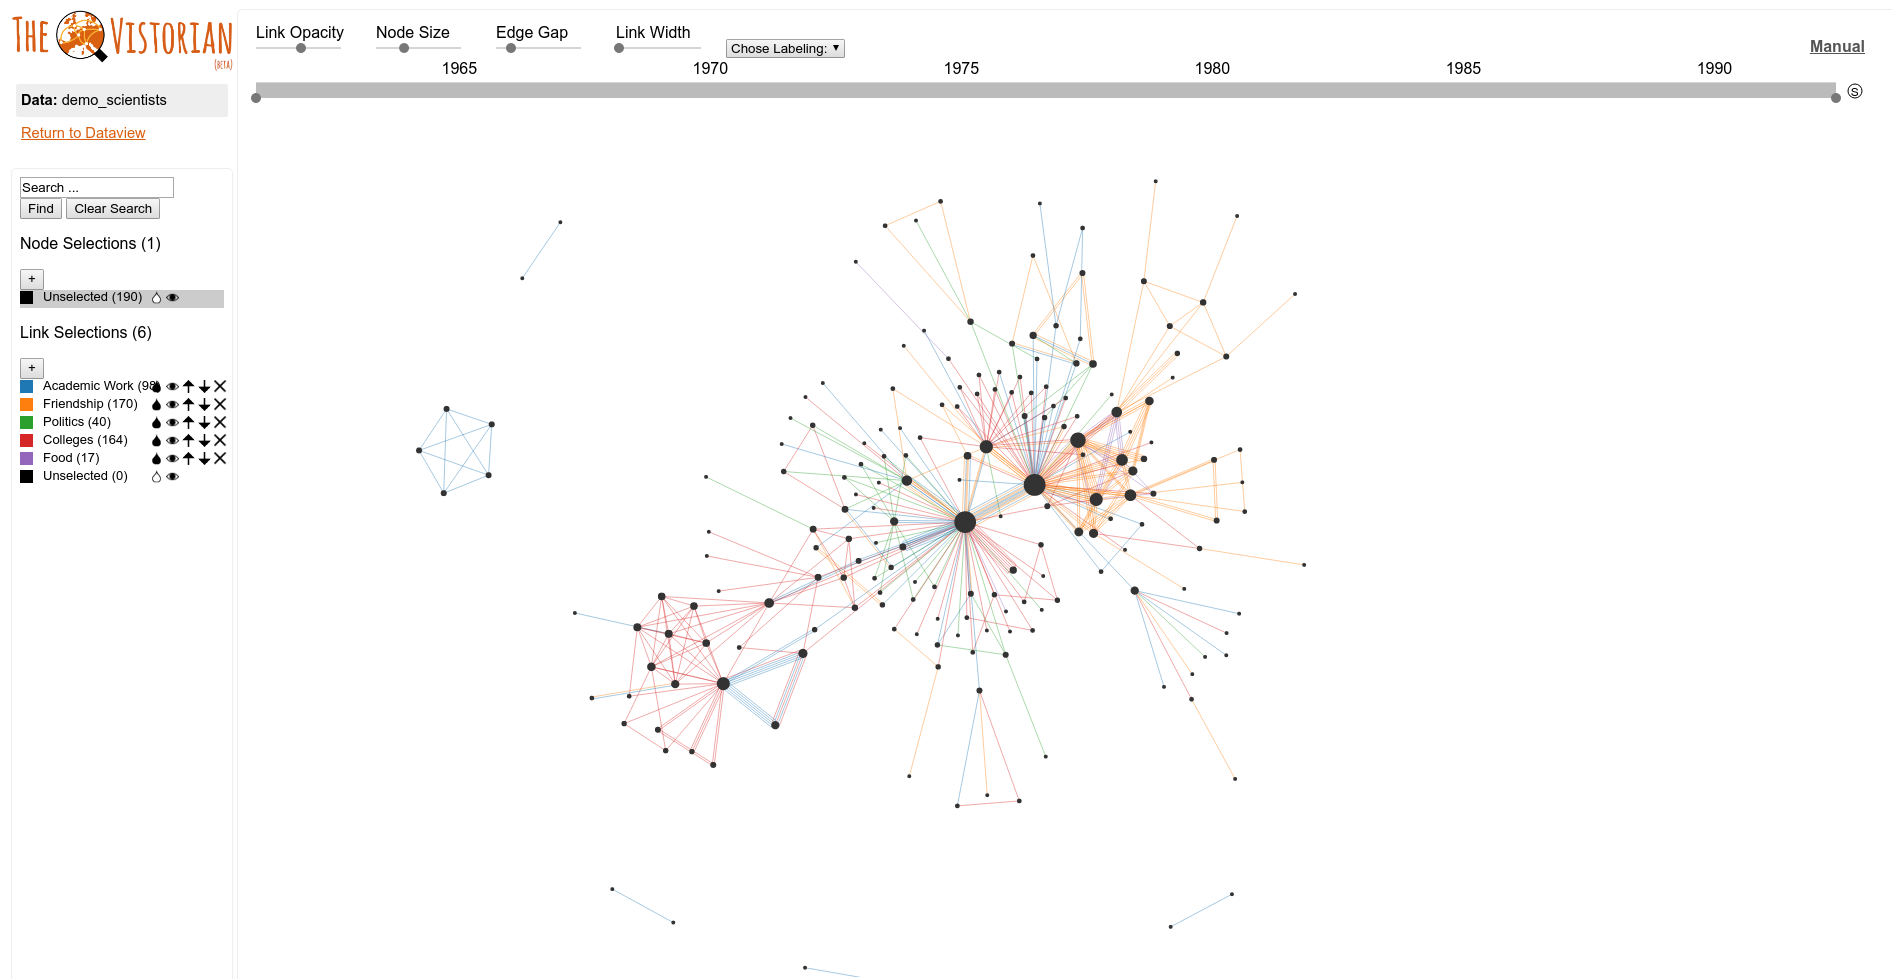
\includegraphics[trim={0 0 0 0}, width=140mm]{./Figures/vistorianOriginal.png}
\end{center}

More details are given in the visualization manual \cite{vismanual} but a summary of the key aspects is provided below.
This project will focus on the ‘Node-link’ visualisation specifically. The node-link diagram is composed of nodes as points and edges as straight lines. The positions of nodes are kept the same for all time-frames, making it easier to visualise \cite{tsotaivg}. It's also simple and intuitive.
%-Node-link is worse than matrix representation when over 20 nodes \cite{acotrogunlambr}.\newline
%-Node-link history and development, why I'm using this one.\newline
At the top of the network page is a time-slider. Adjusting this time slider filters the links shown if they are not present in that window. A force-directed layout is used, meaning that nodes with many common neighbours are drawn close to each other and nodes with fewer connections are moved to the edges. Node size is used to indicate the node degree and line colour indicates a specific type of relation. Edges are defined as the direct links between nodes and only exist during at most one time-frame, whereas a nodepair is active if any edge is present between two nodes - meaning they can exist during multiple time-frames provided there is at least one edge linking the nodes. In The Vistorian the network is split into discrete time-frames where each time-frame represents some change happening in the network. 






%%%%%%%%%%%%%%%%%%%%%%%%%%%%%%%%%%%%%%%%%%%%%%%%%%%%%%%%%%%%%%%%%%%%%%%%%%%%%%%%
%2345678901234567890123456789012345678901234567890123456789012345678901234567890
%        1         2         3         4         5         6         7         8
% THESIS CHAPTER

\chapter{Work Undertaken}

% short summary of the chapter
\section*{Measures}

\section*{Summary}
short summary of the chapter.

\section{Labelled UI and Explanation}
Blah, pictures, talk about some high level decisions and poit out key parts.

\section{Solving the problem}
Blah, pictures, talk about some high level decisions and poit out key parts.

\section{Network Choice}
Networks vary enormously. There are applications from communications to city planning and counter terrorism to the nervous system.[source] Solving the Dynamic Network interpretation problem could feasibly be done on any type of network. For the purposes of this report, a social network was used. Social networks are readily understood and require virtually no domain knowledge, compared with say, biological networks.[source] Since this project aims to tackle dynamic network interpretation, using a simple network as a baseline ensures that difficulties in comprehension aren’t just inherent to the domain but the network itself. Social networks also tend to be comparatively small. (The largest social network is probably facebook so 1-2 billion nodes?)[source]. The network used is small. There are also a variety of existing networks that could be used to test against.

Social network analysis provides a novel window by allowing the impacts to be quantified at the individual level, and the links between past, current and future behaviour to be carried across contexts. <https://besjournals.onlinelibrary.wiley.com/doi/pdf/10.1111/1365-2656.12764>


\section{The Databar}

\begin{center}
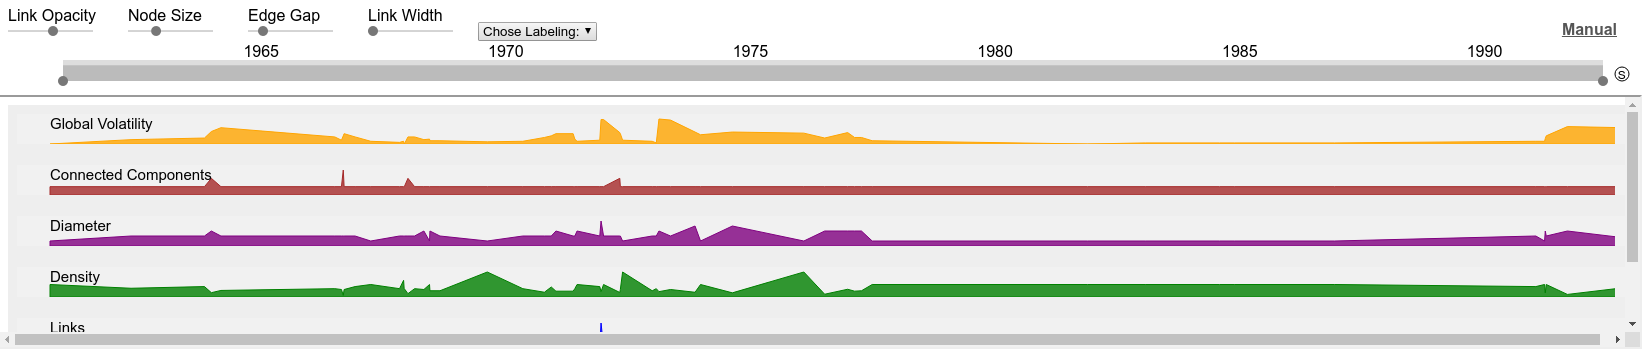
\includegraphics[trim={0 0 0 0}, width=140mm]{./Figures/databar.png}
\end{center}

The Databar holds the global visualisation graphs. I decided to place it along the top of the window because it would line up nicely with the pre-existing timeline which could then double as the x-axis label - saving valuable screen space.
The databar is highly interactive. Each graph is initially collapsed and can then be expanded by clicking.
\begin{center}
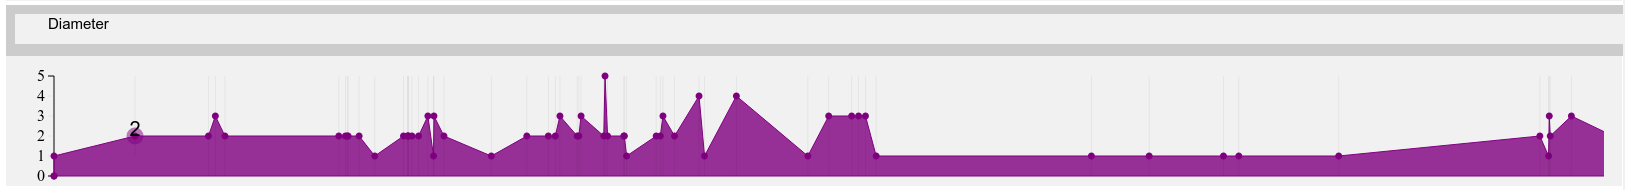
\includegraphics[trim={0 0 0 0}, width=140mm]{./Figures/diameterGraph.png}
\end{center}
Moving the mouse across the screen causes a cursor to track along the ridgeline of the graph. the y-label at that point is shown on the tracker.
\begin{center}
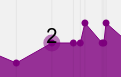
\includegraphics[trim={0 0 0 0}, width=35mm]{./Figures/ridgeTracker.png}
\end{center}
The vertical lines indicate a timestep/change in the graph. This can be useful for comparing graphs vertically and for easily finding time periods of high or low activity.
Finally, graphs can be reordered for easy comparison using click and drag.

\section{Measures and Visualisations}


%%%%%%%%%%%%%%%%%%%%%%%%%%%%%%%%%%%%%%%%%%%%%%%%%%%%%%%%%%%%%%%%%%%%%%%%%%%%%%%%%%%%%%%%%%%%%%%%%%%%%%%%%%%%%%%
%VOLATILITY
%%%%%%%%%%%%%%%%%%%%%%%%%%%%%%%%%%%%%%%%%%%%%%%%%%%%%%%%%%%%%%%%%%%%%%%%%%%%%%%%%%%%%%%%%%%%%%%%%%%%%%%%%%%%%%%

\subsection{Volatility}

\subsubsection{Development}
In my literature review I didn’t come across any examples where this specific measure was used or investigated. I felt that there needed to be some measure or score which captured the level of node connection fluctuation such that a node whose connections tended to stay mostly within a fixed set of other nodes would score low but a node whose edges tended to be short lived and with unfamiliar nodes would score high.
Volatility is a local measure and is calculated with respect to a set start time and end time. Initially it was calculated as the population standard deviation of the number of a node’s connections throughout that time period, effectively the variance in the number of connections.

\begin{center}
population standard deviation = $\sqrt{\frac{1}{N} \sum_{i=1}^N (x_i - \overline{x})^2}$
\end{center}

Examples are given below.


\begin{center}
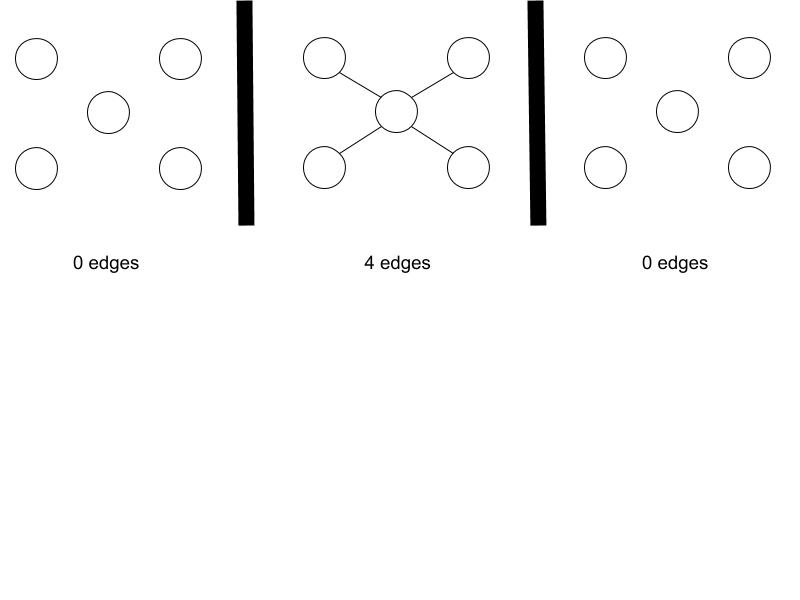
\includegraphics[trim={0 10cm 0 -1cm}, width=120mm]{./Figures/volatility1.jpg}

$N = 3$

$\overline{x} = \frac{4 + 0 + 0}{3} = \frac{4}{3}$

$volatility =\frac{1}{3}\times((0 - \frac{4}{3})^2 + ((4 - \frac{4}{3})^2) + (0 - \frac{4}{3})^2) $

$volatility = 1.89$

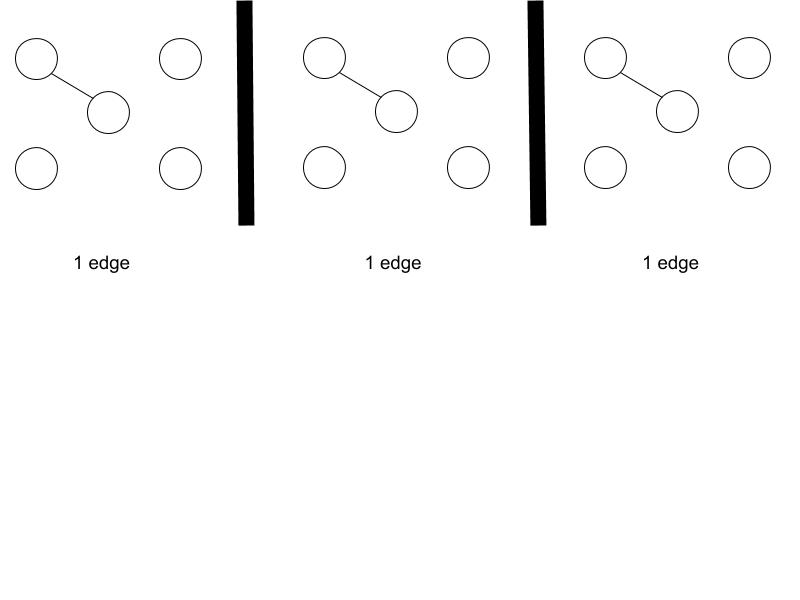
\includegraphics[trim={0 10cm 0 -1cm}, width=120mm]{./Figures/volatility2.jpg}

$N = 3$

$\overline{x} = \frac{1 + 1 + 1}{3} = 1$

$volatility =\frac{1}{3}((1 - 1)^2 + ((1 - 1)^2) + (1 - 1)^2) $

$volatility = 0$
\end{center}

This approach appeared to work quite well - changes in edges results in a higher volatility whereas no changes results in 0 volatility.

However the problem with this approach is that it maintains no ‘memory’ of which edges were previously connected, consider the example below.
\begin{center}
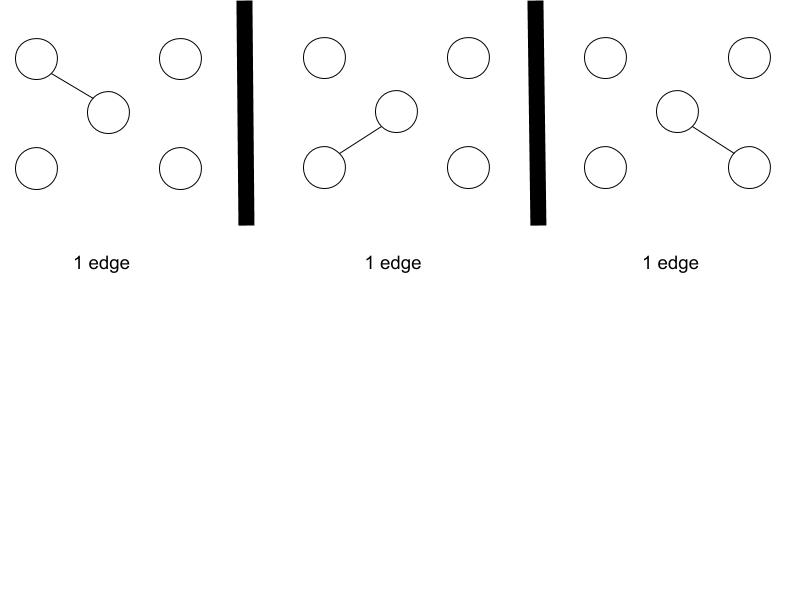
\includegraphics[trim={0 10cm 0 -1cm}, width=120mm]{./Figures/volatility3.jpg}
\end{center}

The volatility will still be 0 despite the edge changing since only the number of edges is taken into account.
To fix this we give edges unique ids and store a binary value tracking which edges are present at each time frame and then sum the standard deviations of these. Example below <I THINK THIS IS INCORRECT AND 2 SHOULDN'T BE THERE:

\begin{center}
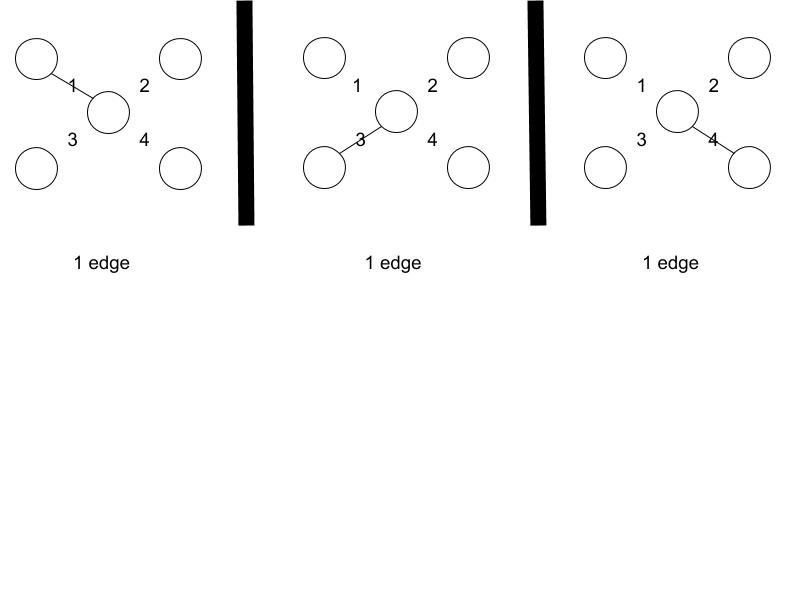
\includegraphics[trim={0 10cm 0 -1cm}, width=120mm]{./Figures/volatility4.jpg}
\end{center}

We store an object mapping edge:[binary value indicating presence during timestep at index].
\begin{center}
\{1:[1, 0, 0], 2: [0, 0, 0], 3: [0, 1, 0], 4: [0, 0, 1]\}
\end{center}
We then calculate volatility as the average of the standard deviations of the object values.
\begin{center}
$volatility = \frac{std([1,0,0]) + std([0,0,0]) + std([0,1,0]) + std([0,0,1])}{4}$

$volatility = 0.35$
\end{center}

<Something about why that data structure makes sense despite the rather large space complexity, it doesn't quite - you could just keep a counter for each edge so if counter was 4 and timesteps were 5 you would do std([1,1,1,1,0]) which would be esay to code - or could be further optimised?, ask BB about this.>

\subsubsection{Vistorian Implementation}
Whilst this solution would work well in a general case it unfortunately works poorly in The Vistorian as edges only appear once. To fix this we instead use node-pairs. 
Volatility in The Vistorian indicates the variance in the number of letters sent and received by a node in a given period. This is useful in the Vistorian because it allows us to see if one contact was rapidly sending or receiving messages to or from new contacts, or if they maintained fairly constant communication with a select number. 

\subsubsection{Visualisation Method}
For visualisation ‘spikes’ are used, where more spikes indicates higher volatility. Other methods were considered, vibration matches with the mental image of volatility but would be too distracting to the eye. Dotted rings with larger diameter indicating higher volatility were considered but had too much potential for confusing overlap. Colours were originally used but could be misconstrued as relating to the edge colours. 

\subsubsection{Further Applications}
Volatility could have broad applications in other domains where dynamic networks are used. 
\newline\newline
Say a system administrator was conducting a post-mortem of an attack on a network using a dynamic network analysis tool to determine which nodes were potentially behaving maliciously. One measure useful in determining an anomaly in a network is the number of successfully established TCP connections in a time interval \cite{fnpfid}. A malicious port scan usually sends a relatively small number of packets to a large number of hosts on a network \cite{fnpfid}. If a similar volatility measure was implemented in this dynamic network analysis tool and TCP connections were considered to be edges it would be very easy for the system administrator to spot particularly volatile, or spiky, nodes.
\newline\newline
Whilst investigating different proteins in protein-protein interaction networks and their impact on the development and progression of hepatocellular carcinoma (HCC) after hepatitis C virus infection the protein core ESR1, which interacted with most of the nodes in the randomly selected sub-network, was shown to be associated with an increased HCC risk \cite{acaotdbnihih}. Using volatility as a measure while performing this anaylsis would have immediately highlighted the ESR1 protein as highly volatile and worthy of further investigation.

%%%%%%%%%%%%%%%%%%%%%%%%%%%%%%%%%%%%%%%%%%%%%%%%%%%%%%%%%%%%%%%%%%%%%%%%%%%%%%%%%%%%%%%%%%%%%%%%%%%%%%%%%%%%%%%
%NUMBER OF LINKS
%%%%%%%%%%%%%%%%%%%%%%%%%%%%%%%%%%%%%%%%%%%%%%%%%%%%%%%%%%%%%%%%%%%%%%%%%%%%%%%%%%%%%%%%%%%%%%%%%%%%%%%%%%%%%%%
\subsection{Number of links}
\subsubsection{Summary}
Simply the number of edges. This gives a quick idea of the degree of activity during a time frame. 

\subsubsection{Reasons for Selection}
The number of edges is one of the most basic measures. However it aids understanding of the network considerably as it provides perhaps the simplest way of understanding the overall activity of the network, keeping cognitive load low while still improving understanding considerably.

\subsubsection{Vistorian Implementation}
This is useful in the Vistorian because the number of messages sent in each given time frame can quickly be seen.
\subsubsection{Visualisation}
\subsubsection{Further Applications}


%%%%%%%%%%%%%%%%%%%%%%%%%%%%%%%%%%%%%%%%%%%%%%%%%%%%%%%%%%%%%%%%%%%%%%%%%%%%%%%%%%%%%%%%%%%%%%%%%%%%%%%%%%%%%%%
%NUMBER OF CONNECTED NODES
%%%%%%%%%%%%%%%%%%%%%%%%%%%%%%%%%%%%%%%%%%%%%%%%%%%%%%%%%%%%%%%%%%%%%%%%%%%%%%%%%%%%%%%%%%%%%%%%%%%%%%%%%%%%%%%
\subsection{Number of connected nodes}
\subsubsection{Summary}
The number of nodes with at least one edge in the given period.

\subsubsection{Reasons for Selection}
Like the number of edges, the number of connected nodes is also a very basic measure. However it gives an easily interpretable sense of the number of actors at a given time. Knowing if activity is high because there are multiple actors or because those actors are each very active is important to be able to distinguish. As it is a simple measure it also keeps cognitive load low while still improving understanding considerably.

\subsubsection{Vistorian Implementation}
In the Vistorian this gives an idea of the number of people involved at each time frame. 

\subsubsection{Visualisation}
\subsubsection{Further Applications}

%%%%%%%%%%%%%%%%%%%%%%%%%%%%%%%%%%%%%%%%%%%%%%%%%%%%%%%%%%%%%%%%%%%%%%%%%%%%%%%%%%%%%%%%%%%%%%%%%%%%%%%%%%%%%%%
%DIAMETER
%%%%%%%%%%%%%%%%%%%%%%%%%%%%%%%%%%%%%%%%%%%%%%%%%%%%%%%%%%%%%%%%%%%%%%%%%%%%%%%%%%%%%%%%%%%%%%%%%%%%%%%%%%%%%%%
\subsection{Diameter}
\subsubsection{Summary}
The longest of all shortest paths in the network. This was implemented using [HOW I DID IT/algorithm] Diameter gives a sense of the interconnectedness of a network.

\subsubsection{Reasons for Selection}
Diameter is particularly important in social networks. The commonly known six-degrees of separation theory https://www.jstor.org/stable/pdf/2786545.pdf?acceptTC=true effectively states that if one were to make a social networks of all humans, the expected diameter would be 6. In a dynamic context... 

\subsubsection{Vistorian Implementation}
In The Vistorian the diameter gives a sense of social distance or degrees of separation between individuals in a ‘conversation’. <may need defined> 
\subsubsection{Visualisation}
\subsubsection{Further Applications}

%%%%%%%%%%%%%%%%%%%%%%%%%%%%%%%%%%%%%%%%%%%%%%%%%%%%%%%%%%%%%%%%%%%%%%%%%%%%%%%%%%%%%%%%%%%%%%%%%%%%%%%%%%%%%%%
%DENSITY
%%%%%%%%%%%%%%%%%%%%%%%%%%%%%%%%%%%%%%%%%%%%%%%%%%%%%%%%%%%%%%%%%%%%%%%%%%%%%%%%%%%%%%%%%%%%%%%%%%%%%%%%%%%%%%%
\subsection{Density}
\subsubsection{Summary}
Density here is defined as (THIS FORMULA). It gives a sense of connectedness at a given period of time. Only nodes with at least one edge are counted. Essentially, if every node is connected to every other node then density will be 1. 

\subsubsection{Reasons for Selection}
Density is used as one of the 7 measures because it gives the user an overview of how interconnected the graph is at a given point and how that varies over time. Since the goal is to provide as much information about the behaviour of the graph as possible using as few measures as possible it is important that information overlap from different measures is minimised. An overview of density can't be easily gathered from observing the graph and it can't be easily extrapolated from the other selected methods.

\subsubsection{Vistorian Implementation}
We define an active node as node that has sent or received a letter during a time frame. In The Vistorian a density of 1 at a time frame means that every  active node during that time frame has either sent or received a letter from every other active node.

\subsubsection{Visualisation}
Density is visualised in the DataBar along with the other global methods. This is detailed in <a>.

\subsubsection{Further Applications}
<a>.

%%%%%%%%%%%%%%%%%%%%%%%%%%%%%%%%%%%%%%%%%%%%%%%%%%%%%%%%%%%%%%%%%%%%%%%%%%%%%%%%%%%%%%%%%%%%%%%%%%%%%%%%%%%%%%%
%NUMBER OF CONNECTED COMPONENTS
%%%%%%%%%%%%%%%%%%%%%%%%%%%%%%%%%%%%%%%%%%%%%%%%%%%%%%%%%%%%%%%%%%%%%%%%%%%%%%%%%%%%%%%%%%%%%%%%%%%%%%%%%%%%%%%
\subsection{Number of connected components}
\subsubsection{Summary}
A connected component is a full group of nodes connected by edges. This measure is simply the number of discrete connected components.
Figure below has two connected components.

\begin{center}
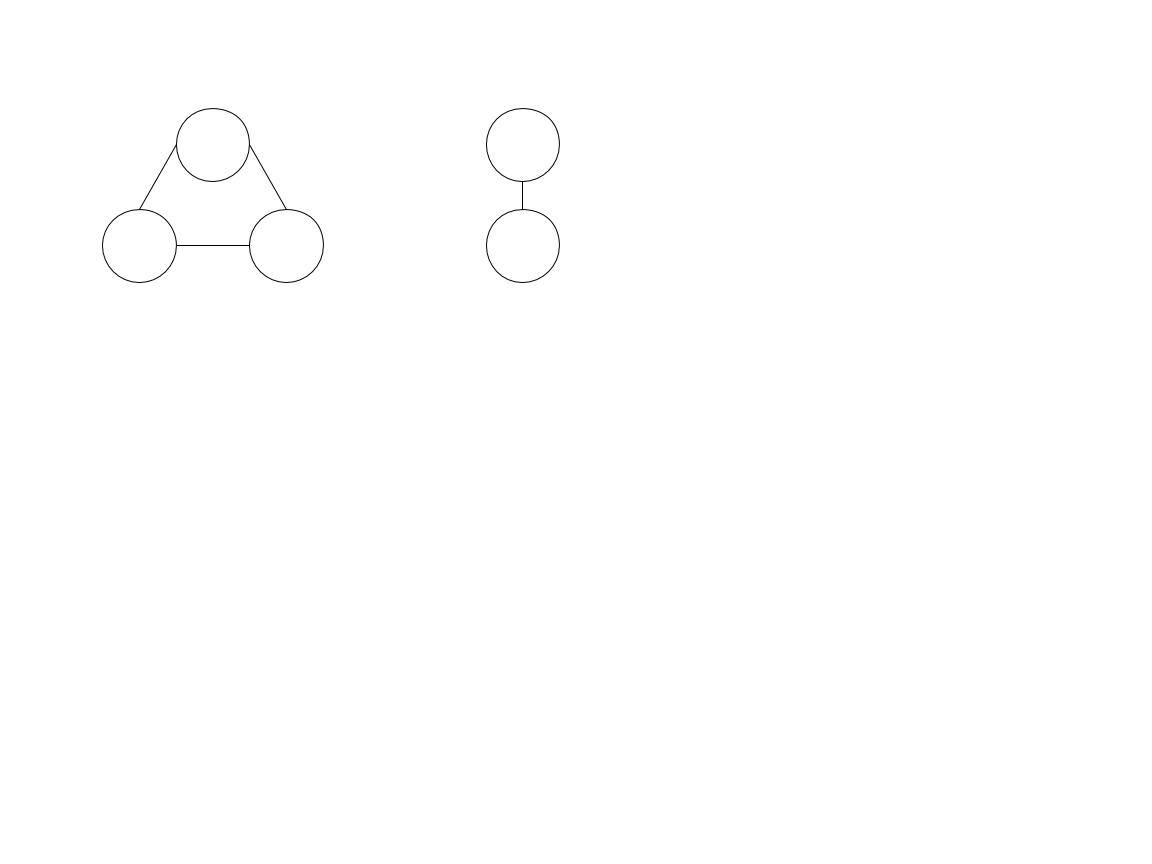
\includegraphics[trim={0cm, 20cm, -10cm, 0cm}, width=180mm]{./Figures/connectedComponents1.jpg}
\end{center}

\subsubsection{Reasons for Selection}
\subsubsection{Vistorian Implementation}
In The Vistorian, this measure can be interpreted as the number of distinct conversations happening during a given chunk of time. 
Should I provide details of the algorithm?

\subsubsection{Visualisation}
\subsubsection{Further Applications}

%%%%%%%%%%%%%%%%%%%%%%%%%%%%%%%%%%%%%%%%%%%%%%%%%%%%%%%%%%%%%%%%%%%%%%%%%%%%%%%%%%%%%%%%%%%%%%%%%%%%%%%%%%%%%%%
%CENTRALITY
%%%%%%%%%%%%%%%%%%%%%%%%%%%%%%%%%%%%%%%%%%%%%%%%%%%%%%%%%%%%%%%%%%%%%%%%%%%%%%%%%%%%%%%%%%%%%%%%%%%%%%%%%%%%%%%
\subsection{Centrality}
\subsubsection{Summary}
Centrality is a local measure. The specific implementation used is betweenness centrality. 

\subsubsection{Reasons for Selection}

\subsubsection{Vistorian Implementation}
Centrality is 

\subsubsection{Visualisation}
\subsubsection{Further Applications}



%%%%%%%%%%%%%%%%%%%%%%%%%%%%%%%%%%%%%%%%%%%%%%%%%%%%%%%%%%%%%%%%%%%%%%%%%%%%%%%%
%2345678901234567890123456789012345678901234567890123456789012345678901234567890
%        1         2         3         4         5         6         7         8
% THESIS CHAPTER

%\section*{Visualisations}

% short summary of the chapter









%%%%%%%%%%%%%%%%%%%%%%%%%%%%%%%%%%%%%%%%%%%%%%%%%%%%%%%%%%%%%%%%%%%%%%%%%%%%%%%%
%2345678901234567890123456789012345678901234567890123456789012345678901234567890
%        1         2         3         4         5         6         7         8
% THESIS CHAPTER

\section*{Points of Interest}

% short summary of the chapter
\section*{Summary}
To further enhance network understanding, "Points of Interest" on the graph are shown. These are points where there are sudden changes or notable outliers across several measures during the same time frame.

\section{Background}
One approach that was considered was to use Shift Detection or Step Detection\cite{sd}. However these methods tended to be designed for noisy data. Since the measures tend to produce little noise <cite?> a simpler method can be used.

We use Tukey Fences to spot outliers. David C. Hoaglin in John W. Tukey and Data Analysis \cite{jwtada} states that Exploratory Data Analysis\cite{eda} uses "fences" to flag possible outliers. These are based on the "hinges," HL and HU, which are approximate quartiles of the batch. He goes on to say that the basic idea is to calculate the H-spread, $d_H = H_U - H_L$, and lay off a multiple of it below $H_L$ and above $H_U$: 

\begin{equation}
 H_L-kd_H \, \, and \, \, H_U + kd_H.
\end{equation}


He continues to say that the limited preliminary edition (Tukey, 1970c) used k = 1.0 for the "side values" and k = 1.5 for the "three-halves values." By the first edition (Tukey, 1977a) the constants had changed a lot, to k = 1.5 for the "inner fences" and k = 3.0 for the "outer fences," with the labels "outside" and "far out," respectively, for data values beyond them.

Finally he states that the aim was not to have a formal rule for declaring an observation an outlier, but to call attention to such data for further investigation. The values of k have remained at 1.5 and 3.0, and the "inner fences" naturally see more use in practice. 


<diagram>


Since the goal is not to formally rule on outliers, this fits nicely with what is required in the Vistorian (ew).



THOUGHTS FROM MEETING

Met with 5 experts. Positive reaction towards the measure visualisations and positive reaction to volatiltiy, towards it's applications and how it as a concept could be applied or modified.
Gill mentioned it could be called promiscuity.
5 of my measures overlapped with theirs - size/number of nodes, number of edges, diameter, density, degree centrality. I don't have Size of Largest Component or the clustering coefficient or Average Path Length. "Sleeping Beauty Papers" in citation networks was mentioned as a possible aspect or direction for volatility. Social Capital was also mentioned - more diverse connections give a richer...? Some way of comparing new links with old links, effectively what I'm doing but perhaps a new way of thinking about it. Tom Schneider, theory on membership. Selecting a subgraph and doing the analysis on that could be very interesting and useful. Could highlight more ephemeral contributions? 
General positive and curious reaction, spurred new ideas and focused the direction to take I think. Very validating to know that this is useful as is. 

- When to stop coding
- What to prioritise (volatility speedup, points of interest, bugfixing, UI, ...)
-Which things they mentioned should be implemented?
-...
%%%%%%%%%%%%%%%%%%%%%%%%%%%%%%%%%%%%%%%%%%%%%%%%%%%%%%%%%%%%%%%%%%%%%%%%%%%%%%%%
%2345678901234567890123456789012345678901234567890123456789012345678901234567890
%        1         2         3         4         5         6         7         8
% THESIS CHAPTER

\chapter{Further Work}
\label{chap:third}
\ifpdf
    \graphicspath{{Chapter3/Figures/PNG/}{Chapter3/Figures/PDF/}{Chapter3/Figures/}}
\else
    \graphicspath{{Chapter3/Figures/EPS/}{Chapter3/Figures/}}
\fi


% short summary of the chapter
\section*{Summary}
Further work, other parts.
\section{Section 1} 
\label{sec:gv1}


\appendix
%%%%%%%%%%%%%%%%%%%%%%%%%%%%%%%%%%%%%%%%%%%%%%%%%%%%%%%%%%%%%%%%%%%%%%%%%%%%%%%%%
%2345678901234567890123456789012345678901234567890123456789012345678901234567890
%        1         2         3         4         5         6         7         8
% THESIS APPENDIX

\chapter{Gesture Vocabulary} 
\label{chap:appendixA}


\begin{figure}
    \centering
    \includegraphics[width=0.8\textwidth]{Chapter4/Figures/Figures/gv.PNG}
    \caption{Proposed gesture vocabulary}
    \label{fig:gs}
\end{figure}


%\chapter{Survey}
\label{chap:appendixB}


%\begin{figure}
%\setboolean{@twoside}{false}
% Uncomment the follow line to show the survey
\includepdf[pages=1-,scale=0.8,pagecommand={}]{Appendix2/gbhri3_format.pdf}
%\end{figure}

%\begin{figure}
 %\centering 
 %\includegraphics{Appendix2/gbhri3_format.pdf}
%\end{figure}
%\bibliographystyle{Classes/RoboticsBiblio}    % bibliography style
\bibliographystyle{ieeetr}
\renewcommand{\bibname}{References}           % change default name Bibliography to References
\bibliography{References/references}          % References file
\addcontentsline{toc}{chapter}{References}    % add References to contents page
%\addcontentsline{toc}{section}{References}
\nocite{*}
\end{document}
